\documentclass[conference]{IEEEtran}
\usepackage[T1]{fontenc}
\usepackage{mathptmx}
\usepackage{amsmath}
\usepackage{graphicx}
\usepackage{booktabs}
\usepackage{array}
\usepackage{url}
\usepackage[hidelinks]{hyperref}

\begin{document}

\title{Instruction and Data Memory Hierarchy:\\Four Memory Organisations around a\\Five-Stage RV32I Pipeline}

\author{\IEEEauthorblockN{Shourya Bafna (2401010444), Daksh Batra (2401010138), Aditya Bhardwaj (2401020007),\\Om Yadav (2401010309), Prajjwal Tripathi (2401010331)}
\IEEEauthorblockA{Newton School of Technology, Rishihood University, Sonipat, Haryana, India\\
Modern Computer Architecture, Project 9 (Section D)}}

\maketitle

\begin{abstract}
A processor fetches an instruction every cycle and, for loads and stores, also reads or writes data. Whether those two streams share one memory port, have separate memories, or are filtered through caches decides how often the pipeline waits. We built a five-stage pipelined RV32I processor in Verilog with separate instruction and data ports and attached it, unchanged, to four memory organisations: von Neumann (one shared memory), Harvard (separate memories), split L1 instruction and write-back data caches over a shared main memory, and a unified L1 cache. Six benchmarks were run on each system while main-memory wait states were swept from 0 to 8. With zero-wait memory, the Harvard system is the fastest (geometric-mean CPI 1.45 against 1.61 for von Neumann), because the shared port turns every load and store into a stalled fetch. Once main memory needs four wait states, split caches run 3.1 times faster than von Neumann (CPI 2.31 against 7.18), and 4.5 times faster at eight. A split cache beats a unified cache of the same size except where pooling capacity lets a working set fit. The split-cache system also needs FENCE.I for self-modifying code, which a test demonstrates. Every simulation is checked instruction by instruction against a Python reference simulator: 480 simulations, including 30 random programs, pass, and seven deliberately injected faults are all caught.
\end{abstract}

\begin{IEEEkeywords}
Harvard architecture, von Neumann architecture, memory hierarchy, cache, pipelining, RISC-V, Verilog, co-simulation
\end{IEEEkeywords}

% =====================================================================
\section{Introduction}

A pipelined processor touches memory in two places. The fetch stage reads one instruction every cycle, and the memory stage reads or writes data for every load and store. When both go through a single memory port they collide, and one must wait: Hennessy and Patterson call this a structural hazard~\cite{hp-quant}, and Backus called the single channel between processor and memory the von Neumann bottleneck~\cite{backus}. A Harvard organisation gives instructions and data separate memories so that both accesses proceed at once. Real processors go one step further and put separate instruction and data caches in front of one shared main memory, which keeps the two-port view at the top of the hierarchy and a single, larger memory below it~\cite{hp-quant,smith}.

Project~9 asks for a Harvard-style memory organisation with separate instruction and data paths, a simple processor to drive it, and a comparison with a shared-memory organisation. We aimed for a comparison that would also hold for a real pipeline and a real memory, and made four contributions:
\begin{enumerate}
    \item A five-stage pipelined RV32I core with forwarding, load-use and branch hazard handling, and memory ports that tolerate any number of wait states. Every empty pipeline slot records why it is empty, so each run produces an exact breakdown of where its cycles went.
    \item Four memory organisations around that core, built from shared components (main memory with configurable wait states, a direct-mapped write-back cache, an arbiter, an address decoder and read/write control): von Neumann, Harvard, split L1 caches over a shared main memory, and a unified L1 cache.
    \item A verification flow that compares every retired instruction, register write and store with a Python reference simulator, for six benchmarks, four directed tests and 30 random programs, on every system and in three configurations. Mutation testing shows that the flow catches each of seven injected faults.
    \item Measurements across main-memory latency and cache size, with stall breakdowns, hit rates and memory traffic, and Yosys synthesis results for all four systems.
\end{enumerate}

% =====================================================================
\section{Literature Review}

\subsection{The stored-program machine and its bottleneck}
Von Neumann's 1945 report on the EDVAC described a machine whose single memory holds both the program and its data~\cite{edvac}. One store made programs easy to load and change, and the design became the template for general-purpose computers. Backus later argued that pushing every instruction and operand through one connection to memory limits both performance and the way programs are written~\cite{backus}. Wulf and McKee observed that processor speed had been improving faster than memory speed for years and predicted that memory access time, rather than computation, would come to decide performance; they called this the memory wall~\cite{wulf}.

\subsection{Harvard machines}
The name comes from the Harvard Mark~I, which read its instructions from punched paper tape while its data lived in separate counters~\cite{aiken}. The idea survives wherever an instruction and its operands must be read in the same cycle. Digital signal processors give the instruction stream and the operand streams their own memories and buses so that a multiply-accumulate can fetch an instruction and two operands at once~\cite{dsp}. Microcontrollers do the same; the ARM Cortex-M3, for example, has separate I-Code and D-Code buses to its code memory plus a system bus~\cite{yiu}.

\subsection{Caches: split, unified and coherent}
Smith's survey of cache memories discusses splitting the first-level cache into instruction and data caches: the split doubles the bandwidth available to the pipeline, while a unified cache of the same total size achieves a better hit ratio because capacity is shared as the program needs it~\cite{smith}. Hill and Smith quantified how associativity reduces conflict misses~\cite{hill}, and Jouppi showed how much of a direct-mapped cache's miss rate comes from such conflicts~\cite{jouppi}. Modern processors use split L1 caches over a unified L2 and main memory, a modified Harvard organisation~\cite{hp-quant}. Textbook pipelines assume separate instruction and data memories for the same reason~\cite{ph-riscv}; Harris and Harris make the contrast explicit with a single-cycle processor that uses separate memories and a multicycle processor that shares one~\cite{harris}. Split caches bring a coherence problem: a store that modifies code goes into the data cache, so the instruction cache may keep running the old instruction. RISC-V leaves this to software, which must execute FENCE.I before running modified code~\cite{riscv-spec}.

\subsection{Open RISC-V cores and their verification}
Open-source RISC-V cores show both choices. PicoRV32 uses a single memory interface for fetches and data and averages about four cycles per instruction~\cite{picorv32}; VexRiscv has separate instruction and data buses, normally connected to separate caches~\cite{vexriscv}. Such cores are commonly verified by running the same program on the RTL and on a reference instruction-set simulator such as Spike and comparing the instruction streams~\cite{spike}. Mutation testing~\cite{demillo} checks the checker by injecting faults and confirming that the tests notice them. The textbooks above describe the structural hazard and the split-versus-unified trade-off qualitatively; this project measures both on one pipeline with only the memory organisation changed.

% =====================================================================
\section{Proposed Solution}

\begin{figure*}[t]
\centering
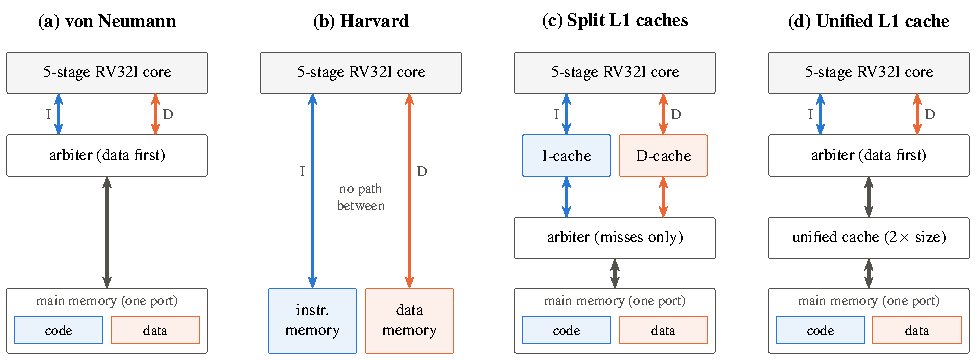
\includegraphics[width=\textwidth]{figures/systems.pdf}
\caption{The four memory organisations. The same core, with an instruction port (I) and a data port (D), is used in every system. Thick grey links are shared by instructions and data; the arbiters give priority to the data access.}
\label{fig:systems}
\end{figure*}

\subsection{System overview}
Fig.~\ref{fig:systems} shows the four systems. All of them use the memory map in Table~\ref{tab:map}, so one program image runs on each. A store to the I/O page sends a value to the output port; the programs report their results that way. The memory sizes match the address map: 16\,KB each for the Harvard instruction and data memories, 32\,KB for the shared main memory, and 1\,KB per split cache (2\,KB unified) unless stated otherwise.

\begin{table}[t]
\centering
\caption{Memory map shared by all four systems}
\label{tab:map}
\footnotesize
\setlength{\tabcolsep}{4pt}
\begin{tabular}{@{}llll@{}}
\toprule
Region & Base address & Size & Use \\
\midrule
Code & \texttt{0x0000\_0000} & 16\,KB & program \\
Data & \texttt{0x1000\_0000} & 16\,KB & data, stack at the top \\
I/O  & \texttt{0x2000\_0000} & 4\,KB & output port (uncached) \\
Other & --- & --- & bus error \\
\bottomrule
\end{tabular}
\end{table}

\begin{figure*}[t]
\centering
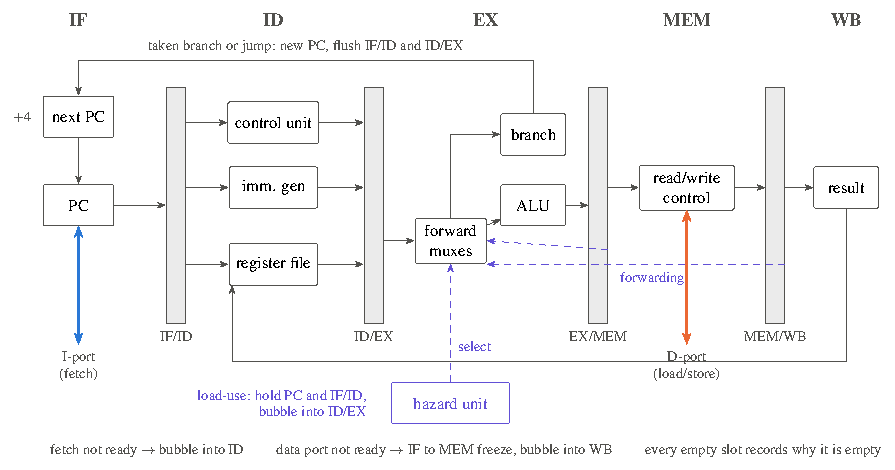
\includegraphics[width=0.92\textwidth]{figures/core.pdf}
\caption{The five-stage RV32I core. Instructions enter through the I-port in IF and access data through the D-port in MEM; the memory system behind the ports differs between the four systems.}
\label{fig:core}
\end{figure*}

\subsection{Five-stage RV32I core}
The core (Fig.~\ref{fig:core}) implements the RV32I base integer instructions~\cite{riscv-spec} except ECALL and EBREAK, plus FENCE and FENCE.I. IF sends the program counter to the I-port. ID decodes the instruction in the control unit, builds the immediate and reads the register file; a register written in WB is passed straight to a read of the same register. EX holds the forwarding multiplexers, the ALU and the branch comparator. MEM holds the read/write control unit and the D-port. WB writes the result back.

Data hazards are handled by forwarding from EX/MEM and MEM/WB; the newer value wins when both match. A load followed directly by an instruction that uses its result costs one stall cycle. Branches and jumps are resolved in EX with static not-taken prediction, so a taken branch flushes the two instructions behind it.

Both ports use the same handshake: the core holds a request until the memory side answers \emph{ready}. When the fetch is not ready, a bubble enters ID and the older instructions continue. When the data access is not ready, IF to MEM freeze and a bubble enters WB. One detail of the freeze took a bug to find (Section~\ref{sec:verification}): the instruction in WB retires during the freeze, so an instruction waiting in EX loses the value it was being forwarded. The ID/EX register therefore re-captures the forwarded operands on every frozen cycle. FENCE.I waits in MEM until the memory system reports that earlier stores are visible to instruction fetch, then refetches the next instruction.

Each pipeline register carries a valid bit and, for an empty slot, the reason it is empty: pipeline fill, fetch not ready, load-use stall, branch flush, data-port wait, or FENCE.I. Exactly one slot reaches WB per cycle, so the cycles of a run divide exactly into retired instructions and the empty slots of each kind.

\subsection{Memory components}
\emph{Main memory} answers a request after a configurable number of wait states $W$, so each word costs $W+1$ cycles; with $W \ge 1$ its read is registered, which lets synthesis use block RAM. If a fetch abandons its request after a branch, the wait restarts for the new address. \emph{Read/write control} turns SB, SH and SW into byte strobes with the data copied onto every lane, and LB, LH, LBU, LHU and LW into extracted, sign- or zero-extended values. The \emph{address decoder} compares the upper address bits with the regions of Table~\ref{tab:map}. In the Harvard system it also enforces the separation: a load or store to the code region is a bus error, because the data side has no path to instruction memory. The \emph{arbiter} shares one port between a data master and an instruction master. The data side wins when both ask, since its request belongs to the older instruction; once a transfer has started, the port stays with that master until the transfer completes.

\subsection{Caches}
The cache is direct-mapped with 16-byte lines, write-back and write-allocate. A hit is answered in the same cycle. A miss first writes the old line back if it is dirty, then reads the new line one word at a time from main memory, then answers the waiting request as a hit. A flush request cleans and invalidates every line; it takes priority over normal requests, because the instruction cache always has a fetch waiting. The same module is used as the L1 instruction cache (never written), the L1 data cache and the unified cache.

\subsection{The four systems}
\emph{Von Neumann}: both ports go through the arbiter to one memory, so every load or store holds up the fetch behind it. \emph{Harvard}: each port has its own memory. \emph{Split L1 caches}: an instruction cache on the I-port and a data cache on the D-port (the I/O page bypasses it), both in front of one main memory through the arbiter, so only misses and write-backs compete. FENCE.I writes back every dirty data-cache line and invalidates the instruction cache. \emph{Unified L1 cache}: the arbiter sits in front of a single cache of twice the size, so the fetch and the data access compete for the cache port even when both would hit.

% =====================================================================
\section{Verification}
\label{sec:verification}

All RTL is Verilog-2005~\cite{verilog}, simulated with Icarus Verilog~\cite{iverilog}. Programs are written in RV32I assembly and assembled by a small assembler written for the project, which is itself checked against 18 hand-worked encodings.

\emph{Unit testbenches} check each block with directed cases: the ALU, register file, program counter, immediate generator and control unit (29 checks); the hazard unit (13); read/write control (20); the address decoder and the arbiter, including the transfer lock (19); and the cache in front of a two-wait-state memory, covering misses, hits, dirty eviction, byte writes, flush and exact cycle counts (16).

\emph{Co-simulation} runs each program on the RTL and on a reference instruction-set simulator written in Python (\texttt{iss.py}), which executes one instruction at a time with no pipeline or cache. The testbench prints every retired instruction with the register it wrote and every store; the two logs must match entry for entry, as must the printed outputs. The reference simulator is itself checked against results computed independently (for example, Python's \texttt{zlib.crc32} for the CRC benchmark). Table~\ref{tab:programs} lists the programs. Each runs on all four systems in three configurations: zero wait states, three wait states, and three-wait memory with tiny 64-byte caches that evict constantly. The same is done for 30 \emph{random programs} of about 400 instructions each. These use a small register pool and a 4\,KB data window, so dependent instructions and cache conflicts are frequent.

\begin{table}[t]
\centering
\caption{Programs. $f_D$ is the fraction of instructions that load or store}
\label{tab:programs}
\footnotesize
\setlength{\tabcolsep}{3pt}
\begin{tabular}{@{}lrrl@{}}
\toprule
Program & Instr. & $f_D$ & What it stresses \\
\midrule
\texttt{collatz} & 59\,591 & 0.000 & branches, registers only \\
\texttt{crc32} & 53\,767 & 0.024 & byte loads, tight loop \\
\texttt{matmul} & 124\,809 & 0.074 & 3\,KB of matrices, calls \\
\texttt{qsort} & 30\,536 & 0.240 & recursion, stack \\
\texttt{listwalk} & 15\,382 & 0.333 & pointer chasing, no locality \\
\texttt{memcpy} & 7\,955 & 0.515 & streaming 8\,KB \\
\midrule
\texttt{isa\_test} & 181 & & 40 self-checks of the ISA \\
\texttt{sep\_test} & 3 & & load from code space \\
\texttt{smc\_test} & 17 & & self-modifying code with FENCE.I \\
\texttt{smc\_nofence} & 16 & & the same without FENCE.I \\
\bottomrule
\end{tabular}
\end{table}

The full flow runs 480 simulations in about 20 seconds on an 11-core laptop, and all of them pass. Two problems found along the way show what the comparison catches. In the first, \texttt{matmul} produced a wrong checksum only on the cached systems. The first mismatch in the commit log was a load that used a stale base register: its producer had been in WB, forwarding to it, when a data-cache miss froze the pipeline, and it retired during the freeze. The fix is the operand re-capture described in Section~III-B. In the second, \texttt{qsort} differed because the program saves a register it never set, which the reference simulator held as zero and the RTL as unknown; the register file now starts at zero, as an FPGA would load it.

\emph{Mutation testing} checks the checks. Table~\ref{tab:mutants} lists seven faults injected one at a time into a copy of the design. The flow caught every one, and an unmodified copy passed.

\begin{table}[t]
\centering
\caption{Injected faults and the first tests that caught them}
\label{tab:mutants}
\footnotesize
\setlength{\tabcolsep}{3pt}
\begin{tabular}{@{}>{\raggedright\arraybackslash}p{0.48\columnwidth}>{\raggedright\arraybackslash}p{0.46\columnwidth}@{}}
\toprule
Fault & Caught by \\
\midrule
EX operands not re-captured during a data wait & qsort, matmul, random programs (cached systems) \\
Forwarding prefers the older value & hazard unit test, five benchmarks \\
Load-use stall removed & hazard unit test, every benchmark \\
Write hit does not mark the line dirty & cache test, benchmarks on cached systems \\
Arbiter does not lock a started transfer & interconnect test \\
Byte store writes the whole word & read/write test, ISA test, random programs \\
FENCE.I does not invalidate the I-cache & \texttt{smc\_test} on split caches only \\
\bottomrule
\end{tabular}
\end{table}

% =====================================================================
\section{Results and Analysis}

\begin{figure*}[t]
\centering
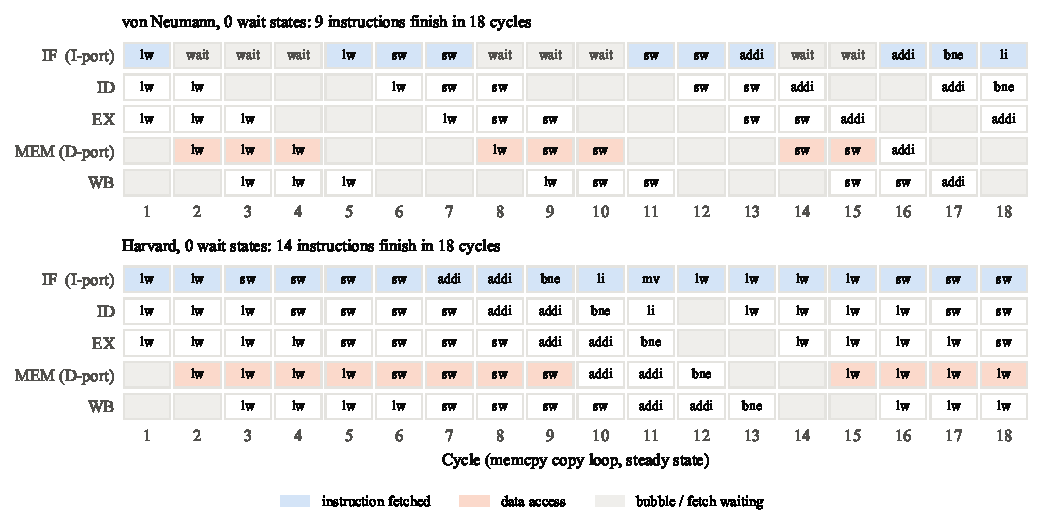
\includegraphics[width=\textwidth]{figures/pipeline_trace.pdf}
\caption{Pipeline occupancy in the \texttt{memcpy} copy loop with zero wait states, taken from the simulation trace. In the von Neumann system each load or store in MEM takes the only port, so IF waits and bubbles follow it down the pipeline; the Harvard system fetches and accesses data in the same cycle.}
\label{fig:trace}
\end{figure*}

\subsection{Zero wait states: the structural hazard}
With single-cycle memory (Table~\ref{tab:cpi}, left), the Harvard system has the lowest geometric-mean CPI, 1.45, against 1.61 for von Neumann: sharing one port costs 11\%. The cost grows with the share of loads and stores. It is zero for \texttt{collatz} and 44\% for \texttt{memcpy}, whose CPI rises from 1.19 to 1.71. Fig.~\ref{fig:trace} shows why: in the copy loop the Harvard pipeline finishes 14 instructions in 18 cycles, the von Neumann pipeline 9.

Caches do not help here. Over zero-wait memory a cache can only add miss penalties: each miss fetches a whole four-word line, so the split-cache system (CPI 1.70) is slower than the plain Harvard system, and the unified cache (1.86) also suffers port conflicts. A cache pays off only when main memory is slower than the cache.

\begin{table}[t]
\centering
\caption{CPI with 0 and 4 main-memory wait states (1\,KB caches)}
\label{tab:cpi}
\footnotesize
\setlength{\tabcolsep}{2.6pt}
\begin{tabular}{@{}lrrrr@{\hskip 8pt}rrrr@{}}
\toprule
 & \multicolumn{4}{c}{0 wait states} & \multicolumn{4}{c}{4 wait states} \\
\cmidrule(lr){2-5}\cmidrule(l){6-9}
Benchmark & VN & Harv. & Split & Unif. & VN & Harv. & Split & Unif. \\
\midrule
collatz  & 1.58 & 1.58 & 1.58 & 1.58 & 5.58 & 5.58 & 1.58 & 1.58 \\
crc32    & 1.51 & 1.49 & 1.49 & 1.53 & 5.71 & 5.59 & 1.51 & 1.61 \\
qsort    & 1.61 & 1.41 & 1.48 & 1.76 & 7.73 & 6.53 & 1.75 & 2.26 \\
matmul   & 1.43 & 1.42 & 1.51 & 1.51 & 6.16 & 5.79 & 1.80 & 1.77 \\
listwalk & 1.87 & 1.67 & 2.18 & 2.43 & 8.73 & 7.06 & 3.89 & 4.32 \\
memcpy   & 1.71 & 1.19 & 2.10 & 2.65 & 10.34 & 7.77 & 5.22 & 5.89 \\
\midrule
geo. mean & 1.61 & \textbf{1.45} & 1.70 & 1.86 & 7.18 & 6.34 & \textbf{2.31} & 2.52 \\
\bottomrule
\end{tabular}
\end{table}

\begin{figure*}[t]
\centering
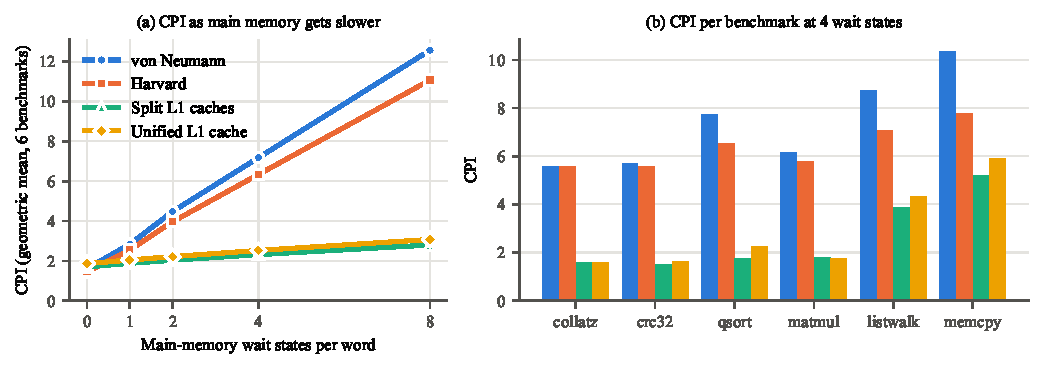
\includegraphics[width=\textwidth]{figures/cpi_latency.pdf}
\caption{(a) Geometric-mean CPI of the six benchmarks as main memory slows down. Without caches every fetch pays the full latency; with caches only misses do. (b) CPI of each benchmark at four wait states.}
\label{fig:latency}
\end{figure*}

\subsection{Slower memory: caches take over}
Fig.~\ref{fig:latency} sweeps main memory from zero to eight wait states. Without caches every instruction fetch pays the full latency, so CPI grows by more than one per wait state for both von Neumann and Harvard. Separate memories still help (Harvard is 12\% faster than von Neumann at eight wait states), but both are far behind the cached systems. With split caches the geometric-mean CPI only rises from 1.70 to 2.80; the speed-up over von Neumann is $1.5\times$ at one wait state, $2.2\times$ at two, $3.1\times$ at four and $4.5\times$ at eight.

\begin{figure*}[t]
\centering
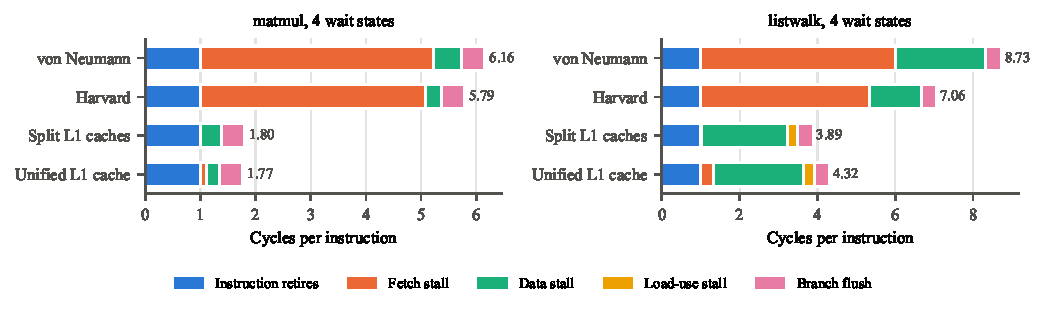
\includegraphics[width=\textwidth]{figures/cpi_stack.pdf}
\caption{Where the cycles go at four wait states, from the empty-slot reasons recorded in the pipeline. Each bar is CPI split into the retiring instruction and the stalls behind it.}
\label{fig:stack}
\end{figure*}

\subsection{Where the cycles go}
Fig.~\ref{fig:stack} breaks CPI into its causes. For \texttt{matmul} without caches, fetch stalls dominate: 4.22 cycles per instruction in the von Neumann system. The split I-cache removes them completely (99.99\% hit rate), and what remains is data-cache misses (0.38) and branch flushes (0.42), which do not depend on memory at all. \texttt{listwalk} is the hard case: it chases pointers through 4\,KB of scattered nodes, so even with caches 2.21 cycles per instruction are spent waiting for data. Load-use stalls appear only in the cached systems, because without caches the fetch is so slow that a load has already finished when its user arrives.

\begin{table}[t]
\centering
\caption{Cache behaviour and main-memory traffic at four wait states}
\label{tab:cache}
\footnotesize
\setlength{\tabcolsep}{3pt}
\begin{tabular}{@{}lrrrrrr@{}}
\toprule
 & \multicolumn{3}{c}{Hit rate (\%)} & \multicolumn{3}{c}{Memory words / instr.} \\
\cmidrule(lr){2-4}\cmidrule(l){5-7}
Benchmark & I\$ & D\$ & Unif. & VN & Split & Unif. \\
\midrule
collatz  & 99.99 & ---   & 99.99 & 1.000 & 0.000 & 0.000 \\
crc32    & 99.99 & 95.00 & 99.71 & 1.048 & 0.006 & 0.019 \\
qsort    & 99.95 & 96.20 & 98.46 & 1.480 & 0.066 & 0.125 \\
matmul   & 99.99 & 83.48 & 99.03 & 1.148 & 0.074 & 0.066 \\
listwalk & 99.98 & 74.02 & 94.79 & 1.666 & 0.428 & 0.471 \\
memcpy   & 99.97 & 75.00 & 91.99 & 2.030 & 0.779 & 0.808 \\
\bottomrule
\end{tabular}
\end{table}

\subsection{Cache behaviour and memory traffic}
Table~\ref{tab:cache} shows why the caches work. The instruction cache hits at least 99.95\% of the time on every benchmark, because all the loops fit in 1\,KB. Data hit rates follow locality: \texttt{memcpy} hits exactly 75\%, one miss per four-word line, since every word is used once; \texttt{listwalk} is close to that only because each node's two words share a line. The caches cut main-memory traffic from 1.0 to 2.0 words per instruction in the von Neumann system to 0.81 or less, and to almost nothing for compute-bound code. \texttt{matmul} shows the weak point of a direct-mapped cache: it writes back 767 dirty lines for only 771 stores, because its three 1\,KB matrices map onto the same cache sets and keep evicting each other.

\begin{figure*}[t]
\centering
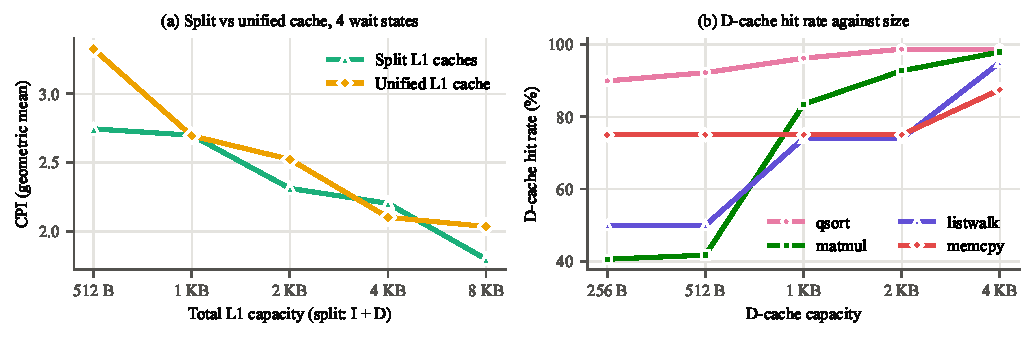
\includegraphics[width=\textwidth]{figures/cache_sweep.pdf}
\caption{(a) Split caches against a unified cache with the same total capacity, at four wait states. (b) Data-cache hit rate against size: hit rates jump when a benchmark's working set starts to fit.}
\label{fig:sweep}
\end{figure*}

\subsection{Split against unified}
Fig.~\ref{fig:sweep}(a) compares the two cache organisations at equal total capacity. The split caches are faster at 512\,B, 2\,KB and 8\,KB, the two tie at 1\,KB, and the unified cache wins at 4\,KB (CPI 2.10 against 2.20). The per-benchmark data shows the trade-off Smith described~\cite{smith}. The unified cache wins only where pooling capacity lets a working set fit that the split data cache cannot hold: \texttt{listwalk}'s 4\,KB list fits in a 4\,KB unified cache but not in a 2\,KB data cache (CPI 2.37 against 3.89). Everywhere else its single port costs it. At 8\,KB, where both organisations hold every working set, the unified cache still has a fetch blocked behind a data access for 0.08 to 1.90 cycles per instruction on the benchmarks that use data, and the split caches are faster on four of the six benchmarks, equal on \texttt{collatz} and 1\% slower on \texttt{memcpy}. Fig.~\ref{fig:sweep}(b) shows the jumps in hit rate as working sets begin to fit.

\subsection{Separation and coherence}
Table~\ref{tab:sep} lists the directed tests. A load from the code region returns an instruction word in every system except Harvard, where the address decoder raises a bus error. The data side cannot even read the program. Self-modifying code shows the other side of separation. With FENCE.I the patched function returns the new value in all systems that allow the store. Without FENCE.I the split-cache system returns the old value, because the new instruction sits dirty in the data cache while the instruction cache keeps the old line. This is the incoherence that RISC-V asks software to resolve with FENCE.I~\cite{riscv-spec}, and the two unified-memory organisations never see it.

\begin{table}[t]
\centering
\caption{Separation and coherence tests}
\label{tab:sep}
\footnotesize
\setlength{\tabcolsep}{3pt}
\begin{tabular}{@{}lllll@{}}
\toprule
Test & VN & Harvard & Split & Unified \\
\midrule
load from code & instruction & bus error & instruction & instruction \\
patch + FENCE.I & 1, 2 & bus error & 1, 2 & 1, 2 \\
patch, no fence & 1, 2 & bus error & \textbf{1, 1 (stale)} & 1, 2 \\
\bottomrule
\end{tabular}
\end{table}

\subsection{Synthesis}
Table~\ref{tab:synth} gives Yosys~\cite{yosys} results for a Xilinx 7-series device with one wait state, so every main memory maps to block RAM. The two systems without caches use about 1\,300 logic LUTs, most of it the core. The caches add their tag logic and multiplexing (about 650 LUTs for the split pair, 1\,200 for the unified cache, whose single port also needs the arbiter on the hit path) and keep their data in LUT RAM. These figures are taken before placement and routing.

\begin{table}[t]
\centering
\caption{Yosys synthesis, Xilinx 7-series, one wait state}
\label{tab:synth}
\footnotesize
\setlength{\tabcolsep}{3pt}
\begin{tabular}{@{}lrrrr@{}}
\toprule
Resource & VN & Harvard & Split & Unified \\
\midrule
Logic LUTs & 1\,296 & 1\,375 & 2\,036 & 2\,514 \\
LUTs used as RAM & 48 & 48 & 560 & 928 \\
Flip-flops & 441 & 498 & 688 & 740 \\
Block RAM (36\,Kb) & 8 & 7.5 & 8.5 & 8 \\
Carry chains & 62 & 64 & 72 & 68 \\
\bottomrule
\end{tabular}
\end{table}

\subsection{Limitations}
Main memory transfers one word per request; a burst transfer would make line refills cheaper and favour caches further. The caches are direct-mapped, so \texttt{matmul} and \texttt{memcpy} suffer conflict misses that a two-way cache would remove~\cite{hill}. The single-cycle cache hit puts the tag comparison on the pipeline's stall path, which is likely to limit clock frequency on an FPGA.

% =====================================================================
\section{Individual Contributions}

Table~\ref{tab:contrib} lists who built what. Each member committed their own files to the project repository, so the commit history shows the same split.

\begin{table}[!h]
\centering
\caption{Individual contributions}
\label{tab:contrib}
\footnotesize
\setlength{\tabcolsep}{3pt}
\begin{tabular}{@{}>{\raggedright\arraybackslash}p{0.25\columnwidth}>{\raggedright\arraybackslash}p{0.71\columnwidth}@{}}
\toprule
Member & Work (design, verification, report) \\
\midrule
Shourya Bafna\newline 2401010444 & Five-stage pipelined core (\texttt{core.v}), hazard unit and its testbench; repository and integration. Report: Sections I, III-B, VI, VII, editing. \\
\addlinespace
Daksh Batra\newline 2401010138 & Program counter, register file, ALU, immediate generator, control unit; datapath testbench. Report: Section II. \\
\addlinespace
Aditya Bhardwaj\newline 2401020007 & Main memory with wait states, write-back cache, read/write control; cache and read/write testbenches. Report: Sections III-C, III-D. \\
\addlinespace
Om Yadav\newline 2401010309 & Address decoder, arbiter, the four system top levels; interconnect testbench. Report: Sections III-A, III-E. \\
\addlinespace
Prajjwal Tripathi\newline 2401010331 & Assembler, reference simulator, random program generator, benchmark and test programs, system testbench; verification, experiment, plotting and synthesis scripts. Report: Sections IV, V. \\
\bottomrule
\end{tabular}
\end{table}

% =====================================================================
\section{Conclusion and Phase II Plan}

We built a five-stage RV32I pipeline and four memory organisations around it, and verified every run against a reference simulator. Separate instruction and data paths matter at every level of the hierarchy. With fast memory, the Harvard system avoids the structural hazard that costs von Neumann 11\% on average and 44\% on a copy loop. With slow memory, split caches over a shared main memory keep the two-port view while sharing one memory, and run up to 4.5 times faster than von Neumann; they also beat a unified cache except where pooled capacity lets a working set fit. That organisation needs FENCE.I for self-modifying code, which a test shows. For Phase~II we plan to place and route the design to measure maximum clock frequency and run it on an FPGA, add burst refills and a two-way set-associative data cache, and pipeline the cache hit to shorten the critical path.

% =====================================================================
\begin{thebibliography}{99}

\bibitem{edvac}
J.~von Neumann, ``First draft of a report on the EDVAC,'' \emph{IEEE Ann. Hist. Comput.}, vol.~15, no.~4, pp.~27--75, 1993. (Reprint of the 1945 report.)

\bibitem{aiken}
H.~H. Aiken and G.~M. Hopper, ``The Automatic Sequence Controlled Calculator---I,'' \emph{Electr. Eng.}, vol.~65, no.~8--9, pp.~384--391, 1946.

\bibitem{backus}
J.~Backus, ``Can programming be liberated from the von Neumann style? A functional style and its algebra of programs,'' \emph{Commun. ACM}, vol.~21, no.~8, pp.~613--641, Aug. 1978.

\bibitem{wulf}
W.~A. Wulf and S.~A. McKee, ``Hitting the memory wall: Implications of the obvious,'' \emph{ACM SIGARCH Comput. Archit. News}, vol.~23, no.~1, pp.~20--24, Mar. 1995.

\bibitem{hp-quant}
J.~L. Hennessy and D.~A. Patterson, \emph{Computer Architecture: A Quantitative Approach}, 6th~ed. Cambridge, MA, USA: Morgan Kaufmann, 2017.

\bibitem{ph-riscv}
D.~A. Patterson and J.~L. Hennessy, \emph{Computer Organization and Design RISC-V Edition: The Hardware/Software Interface}, 2nd~ed. Cambridge, MA, USA: Morgan Kaufmann, 2020.

\bibitem{harris}
S.~L. Harris and D.~Harris, \emph{Digital Design and Computer Architecture: RISC-V Edition}. Cambridge, MA, USA: Morgan Kaufmann, 2021.

\bibitem{smith}
A.~J. Smith, ``Cache memories,'' \emph{ACM Comput. Surv.}, vol.~14, no.~3, pp.~473--530, Sep. 1982.

\bibitem{hill}
M.~D. Hill and A.~J. Smith, ``Evaluating associativity in CPU caches,'' \emph{IEEE Trans. Comput.}, vol.~38, no.~12, pp.~1612--1630, Dec. 1989.

\bibitem{jouppi}
N.~P. Jouppi, ``Improving direct-mapped cache performance by the addition of a small fully-associative cache and prefetch buffers,'' in \emph{Proc. 17th Annu. Int. Symp. Comput. Archit. (ISCA)}, 1990, pp.~364--373.

\bibitem{dsp}
J.~Eyre and J.~Bier, ``The evolution of DSP processors,'' \emph{IEEE Signal Process. Mag.}, vol.~17, no.~2, pp.~43--51, Mar. 2000.

\bibitem{yiu}
J.~Yiu, \emph{The Definitive Guide to ARM Cortex-M3 and Cortex-M4 Processors}, 3rd~ed. Oxford, U.K.: Newnes, 2014.

\bibitem{riscv-spec}
A.~Waterman and K.~Asanovi\'{c}, Eds., \emph{The RISC-V Instruction Set Manual, Volume~I: Unprivileged ISA}, Document Version 20191213, RISC-V Foundation, Dec. 2019.

\bibitem{picorv32}
C.~Wolf, ``PicoRV32: A size-optimized RISC-V CPU,'' GitHub repository. [Online]. Available: \url{https://github.com/YosysHQ/picorv32}

\bibitem{vexriscv}
SpinalHDL, ``VexRiscv: A FPGA friendly 32 bit RISC-V CPU implementation,'' GitHub repository. [Online]. Available: \url{https://github.com/SpinalHDL/VexRiscv}

\bibitem{spike}
RISC-V International, ``Spike RISC-V ISA simulator,'' GitHub repository. [Online]. Available: \url{https://github.com/riscv-software-src/riscv-isa-sim}

\bibitem{demillo}
R.~A. DeMillo, R.~J. Lipton, and F.~G. Sayward, ``Hints on test data selection: Help for the practicing programmer,'' \emph{Computer}, vol.~11, no.~4, pp.~34--41, Apr. 1978.

\bibitem{verilog}
\emph{IEEE Standard for Verilog Hardware Description Language}, IEEE Std 1364-2005, 2006.

\bibitem{iverilog}
S.~Williams, ``Icarus Verilog.'' [Online]. Available: \url{https://steveicarus.github.io/iverilog/}

\bibitem{yosys}
C.~Wolf, ``Yosys Open SYnthesis Suite.'' [Online]. Available: \url{https://yosyshq.net/yosys/}

\end{thebibliography}

\end{document}
